% Paper notes for the Datathon 26 ForteBank case.
% Build from inside research/:   latexmk -pdf paper_notes.tex && latexmk -c
% Add a paper: drop its PDF into papers/, then copy the template at the end of
% the longtable. Each paper is a block of rows; longtable can break the page
% between rows but never inside one, so keep every row shorter than a page.

\documentclass[10pt]{article}
\usepackage[a4paper,landscape,left=12mm,right=12mm,top=11mm,bottom=14mm,footskip=7mm]{geometry}
\usepackage[T1]{fontenc}
\usepackage[default,semibold]{sourcesanspro}
\usepackage{amsmath}
\usepackage{newtxsf}
\usepackage{microtype}
\usepackage[table]{xcolor}
\usepackage{tikz}
\usetikzlibrary{arrows.meta,calc,backgrounds,decorations.pathreplacing}
\usepackage{longtable,booktabs,array}
\usepackage{fontawesome5}
\usepackage{fancyhdr}
\usepackage[hyphens]{url}
\usepackage{hyperref}

% ---------------------------------------------------------------- colours
% Categorical slots and status colours from the dataviz reference palette.
\definecolor{ink}{HTML}{0B0B0B}
\definecolor{ink2}{HTML}{52514E}
\definecolor{muted}{HTML}{8A8984}
\definecolor{grid}{HTML}{E4E3DF}
\definecolor{panel}{HTML}{F5F5F3}
\definecolor{indu}{HTML}{2A78D6}   % induction, slot 1
\definecolor{dedu}{HTML}{EB6834}   % deduction, slot 2
\definecolor{rulec}{HTML}{1BAF7A}  % rules, slot 3
\definecolor{anom}{HTML}{D03B3B}   % status critical: anomaly
\definecolor{good}{HTML}{0CA30C}   % status good
\definecolor{warn}{HTML}{FAB219}   % status warning

\hypersetup{colorlinks=true,linkcolor=ink,urlcolor=indu!80!black,filecolor=indu!80!black,
  pdftitle={Paper notes},pdfsubject={Datathon 26, ForteBank case}}

\pagestyle{fancy}
\fancyhf{}
\renewcommand{\headrulewidth}{0pt}
\fancyfoot[L]{\fontsize{6}{7}\selectfont\color{muted}Paper notes, Datathon 26}
\fancyfoot[R]{\fontsize{6}{7}\selectfont\color{muted}\thepage}

\setlength{\parindent}{0pt}
\setlength{\tabcolsep}{6pt}
\newlength{\papercolw}\setlength{\papercolw}{5.0cm}
\newlength{\desccolw}\setlength{\desccolw}{\dimexpr\textwidth-\papercolw-2\tabcolsep\relax}

\newcommand{\sixpt}{\fontsize{6}{7.2}\selectfont}
\newcommand{\rowhead}[2]{{\small\bfseries\color{muted}#1\quad\color{ink}#2}\par\vspace{5pt}}
\newcommand{\chip}[1]{\tikz[baseline=(c.base)]\node[fill=panel,draw=grid,rounded corners=2pt,
  inner xsep=3pt,inner ysep=1.6pt,font=\sixpt,text=ink2](c){#1};}
\newcommand{\cont}[2]{\begin{minipage}[t]{\linewidth}\raggedright
  {\scriptsize\color{muted}#1}\par{\sixpt\color{muted}part #2}\end{minipage}}
\newcommand{\textcol}[2]{\begin{minipage}[t]{#1}\small\raggedright #2\end{minipage}}

% ---------------------------------------------------------------- tikz
\tikzset{
  >={Stealth[length=4.5pt,width=4pt]},
  flow/.style={->,line width=0.7pt,draw=ink2},
  dflow/.style={->,line width=0.7pt,draw=ink2,dash pattern=on 2.5pt off 1.8pt},
  stage/.style={draw=#1,fill=#1!8,rounded corners=3pt,line width=0.6pt,align=center,
    font=\scriptsize,text=ink,inner sep=3.5pt},
  pill/.style={draw=ink2,fill=white,rounded corners=6pt,line width=0.6pt,
    font=\scriptsize\bfseries,text=ink,inner xsep=6pt,inner ysep=3pt,minimum height=0.5cm},
  card/.style={draw=grid,fill=white,rounded corners=2pt,line width=0.5pt,align=left,
    font=\scriptsize,text=ink,inner sep=3pt,text width=#1},
  lbl/.style={font=\scriptsize,text=ink2,align=center},
  sublbl/.style={font=\sixpt,text=muted,align=center},
  ptitle/.style={font=\scriptsize\bfseries,text=ink,anchor=west},
  rowlab/.style={font=\scriptsize,text=ink,anchor=west},
  rowsub/.style={font=\sixpt,text=muted,anchor=west},
  badge/.style={circle,fill=ink,text=white,font=\sixpt\bfseries,inner sep=0pt,minimum size=0.32cm},
  % cell fill by value, so \fill[c\v] works inside \foreach
  c0/.style={fill=grid}, c1/.style={fill=anom},
  t0/.style={text=ink2}, t1/.style={text=white},
  d0/.style={fill=white,draw=indu,line width=0.6pt}, d1/.style={fill=indu,draw=white,line width=0.6pt},
  fx1/.style={circle,fill=good,text=white,font=\sixpt\bfseries,inner sep=0pt,minimum size=0.3cm},
  fx0/.style={circle,fill=warn,text=ink,font=\sixpt\bfseries,inner sep=0pt,minimum size=0.3cm},
  k1/.style={text=ink}, k0/.style={text=muted},
  tagbase/.style={rounded corners=5pt,font=\sixpt\bfseries,minimum width=1.2cm,inner sep=2.5pt,line width=0.5pt},
  tg-keep/.style={tagbase,fill=panel,draw=grid,text=ink2},
  tg-change/.style={tagbase,fill=indu!12,draw=indu!50,text=ink},
  tg-add/.style={tagbase,fill=rulec!15,draw=rulec,text=ink},
  % stick figures, origin at the feet
  pics/walker/.style={code={
    \fill[ink2] (0,0.285) circle (0.045);
    \draw[ink2,line width=0.6pt,line cap=round,line join=round]
      (0,0.235) -- (0,0.11) -- (-0.045,0) (0,0.11) -- (0.045,0.005)
      (-0.05,0.155) -- (0,0.2) -- (0.05,0.15);
  }},
  pics/skater/.style={code={
    \pic at (0,0.04) {walker};
    \draw[anom,line width=0.9pt,line cap=round] (-0.085,0.02) -- (0.085,0.02);
    \fill[anom] (-0.052,-0.002) circle (0.016) (0.052,-0.002) circle (0.016);
  }},
  pics/cyclist/.style={code={
    \draw[anom,line width=0.55pt] (-0.085,0.05) circle (0.05) (0.085,0.05) circle (0.05);
    \draw[anom,line width=0.55pt,line join=round] (-0.085,0.05) -- (-0.02,0.125) -- (0.055,0.125) -- (0.085,0.05)
      (-0.02,0.125) -- (0,0.05);
    \fill[ink2] (-0.005,0.315) circle (0.045);
    \draw[ink2,line width=0.6pt,line cap=round,line join=round] (-0.01,0.265) -- (-0.02,0.15) (-0.012,0.23) -- (0.055,0.16);
  }},
  pics/vframe/.style={code={
    \draw[draw=muted!70,fill=white,line width=0.45pt,rounded corners=1pt] (-0.36,-0.26) rectangle (0.36,0.26);
    \draw[grid!60!muted,line width=0.4pt] (-0.36,-0.14) -- (0.36,-0.14);
    \pic at (0,-0.14) {#1};
  }},
  pics/vframe2/.style={code={
    \draw[draw=muted!70,fill=white,line width=0.45pt,rounded corners=1pt] (-0.36,-0.26) rectangle (0.36,0.26);
    \draw[grid!60!muted,line width=0.4pt] (-0.36,-0.14) -- (0.36,-0.14);
    \pic at (-0.15,-0.14) {walker};
    \pic at (0.15,-0.14) {skater};
  }},
}
% encoder-decoder glyph centred at (#1,#2)
\newcommand{\netglyph}[2]{%
  \draw[ink2,fill=white,line width=0.6pt,line join=round]
    (#1-0.5,#2+0.32) -- (#1-0.06,#2+0.12) -- (#1-0.06,#2-0.12) -- (#1-0.5,#2-0.32) -- cycle
    (#1+0.5,#2+0.32) -- (#1+0.06,#2+0.12) -- (#1+0.06,#2-0.12) -- (#1+0.5,#2-0.32) -- cycle;}
% horizontal bar with a rounded data end: \hbarr{x0}{y}{length}
\newcommand{\hbarr}[3]{%
  \fill[indu] (#1,#2-0.14) -- ({#1+#3-0.06},#2-0.14) arc[start angle=-90,end angle=0,radius=0.06]
    -- ({#1+#3},#2+0.08) arc[start angle=0,end angle=90,radius=0.06] -- (#1,#2+0.14) -- cycle;}

\begin{document}

\noindent{\fontsize{17}{20}\selectfont\bfseries Paper notes}\hfill
{\scriptsize\color{ink2}Datathon 26, ForteBank cashier-video case, 17 October 2026}\par
\vspace{4pt}
\noindent\begin{minipage}{0.8\textwidth}\small\color{ink2}
One row per paper. Click a title to open the local copy in \texttt{papers/}. I drew the figures
for these notes from each paper's text; they are not copies of the paper's own figures.
Charts with real numbers name the table they come from, and toy examples say so.
\end{minipage}\par\vspace{8pt}

\arrayrulecolor{grid}
\begin{longtable}{@{}p{\papercolw}p{\desccolw}@{}}
\arrayrulecolor{ink}\toprule
{\scriptsize\bfseries Paper} & {\scriptsize\bfseries Method, explained with figures} \\
\arrayrulecolor{grid}\midrule
\endfirsthead
\arrayrulecolor{ink}\toprule
{\scriptsize\bfseries Paper} & {\scriptsize\bfseries Method, explained with figures, continued} \\
\arrayrulecolor{grid}\midrule
\endhead
\arrayrulecolor{ink}\bottomrule
\endlastfoot

% =====================================================================
% 01  AnomalyRuler, ECCV 2024
% =====================================================================
\begin{minipage}[t]{\linewidth}\raggedright
{\fontsize{22}{24}\selectfont\bfseries\color{grid!50!muted}01}\par\vspace{5pt}
{\small\bfseries\href{papers/yang2024_eccv_follow_the_rules.pdf}{Follow the Rules: Reasoning for Video Anomaly Detection with Large Language Models}}\par\vspace{5pt}
{\scriptsize\color{ink2}Yuchen Yang, Kwonjoon Lee, Behzad Dariush, Yinzhi Cao, Shao-Yuan Lo\par
Johns Hopkins University and Honda Research Institute USA\par}
\vspace{4pt}
{\scriptsize\bfseries ECCV 2024}\quad{\scriptsize\color{ink2}method name AnomalyRuler}\par
\vspace{8pt}
{\scriptsize
\href{papers/yang2024_eccv_follow_the_rules.pdf}{\faFilePdf\enspace local copy}\par
{\sixpt\color{muted}\path{papers/yang2024_eccv_follow_the_rules.pdf}}\par\vspace{2pt}
\href{https://www.ecva.net/papers/eccv_2024/papers_ECCV/papers/10568.pdf}{\faGlobe\enspace ECVA open-access PDF}\par\vspace{2pt}
\href{https://mlanthology.org/eccv/2024/yang2024eccv-follow/}{\faBookOpen\enspace ML Anthology page}\par\vspace{2pt}
\href{https://github.com/Yuchen413/AnomalyRuler}{\faGithub\enspace code on GitHub}\par\vspace{2pt}
\href{https://doi.org/10.1007/978-3-031-73004-7_18}{\faLink\enspace doi 10.1007/978-3-031-73004-7\_18}\par}
\vspace{8pt}
\chip{one-class VAD} \chip{few normal shots} \chip{no training}\par\vspace{2pt}
\chip{LLM reasoning} \chip{explains each call}\par
\vspace{10pt}
{\scriptsize\color{ink}\textbf{Why it is here.} It explains each detection by naming a rule and
needs only a few normal clips. Our brief asks for both.}
\end{minipage}
&
\begin{minipage}[t]{\linewidth}
\rowhead{1}{The problem it fixes}
\begin{tikzpicture}[x=1cm,y=1cm]
\node[anchor=west,font=\scriptsize,text=ink2] at (0,0.32) {\faInfoCircle\enspace Scene: a campus walkway where only walking is allowed. The test frame shows one person walking and one skateboarding.};
\foreach \px/\ttl in {0/{a\quad Classic one-class detector},7.25/{b\quad Ask an LLM directly},14.5/{c\quad AnomalyRuler}}{
  \fill[panel,rounded corners=4pt] (\px,0) rectangle ++(7.05,-5.0);
  \node[ptitle] at ({\px+0.2},-0.32) {\ttl};
  \node[anchor=west,font=\sixpt\bfseries,text=muted] at ({\px+0.2},-0.78) {SETUP};
  \node[anchor=west,font=\sixpt\bfseries,text=muted] at ({\px+0.2},-2.82) {TEST};
}
% a
\foreach \k in {2,1,0} \pic[scale=1.2] at ({0.85+\k*0.12},{-1.62+\k*0.1}) {vframe=walker};
\node[sublbl] at (1.0,-2.3) {all normal\\training frames};
\draw[flow] (1.7,-1.6) -- (2.45,-1.6);
\netglyph{3.05}{-1.6}
\node[lbl,anchor=west,align=left] at (3.75,-1.6) {train a network to\\reconstruct normal frames};
\pic[scale=1.2] at (0.85,-3.4) {vframe2};
\draw[flow] (1.4,-3.4) -- (2.45,-3.4);
\netglyph{3.05}{-3.4}
\draw[flow] (3.65,-3.4) -- (4.25,-3.4);
\node[draw=ink2,fill=white,rounded corners=2pt,font=\small\bfseries,text=ink,minimum width=1.05cm,minimum height=0.55cm] at (4.85,-3.4) {0.83};
\node[sublbl] at (4.85,-3.92) {anomaly score};
\node[lbl,anchor=west] at (5.5,-3.4) {\faQuestionCircle\ why?};
\node[anchor=west,font=\scriptsize,text=ink] at (0.2,-4.58) {Needs the full training set and returns a bare number.};
% b
\node[draw=muted,dash pattern=on 2pt off 1.5pt,rounded corners=2pt,font=\scriptsize,text=ink2,text width=6.0cm,align=center,inner sep=5pt] at (10.775,-1.6) {Nothing to set up. The model relies on\\what it picked up in pretraining.};
\pic[scale=1.2] at (8.1,-3.4) {vframe2};
\node[pill] (g4) at (9.85,-3.4) {GPT-4V};
\draw[flow] (8.65,-3.4) -- (g4.west);
\node[card=2.85cm,anchor=west] (sp) at (10.95,-3.3) {Nothing unusual. A regular day in a park: people walking, one person skateboarding.};
\draw[flow] (g4.east) -- (10.95,-3.4);
\node[anchor=north west,font=\scriptsize,text=ink] at (10.95,-3.98) {\textcolor{anom}{\faTimesCircle}\enspace says normal, which is wrong};
\node[anchor=west,font=\scriptsize,text=ink] at (7.45,-4.58) {Its general sense of normal does not fit this scene.};
% c
\foreach \k in {2,1,0} \pic[scale=1.2] at ({15.3+\k*0.12},{-1.62+\k*0.1}) {vframe=walker};
\node[sublbl] at (15.45,-2.3) {a few normal\\frames};
\node[pill] (ind) at (17.2,-1.6) {LLM};
\node[sublbl] at (17.2,-2.05) {induce};
\draw[flow] (16.15,-1.6) -- (ind.west);
\node[card=2.85cm,anchor=west,draw=rulec,line width=0.7pt] (rc) at (18.3,-1.6) {\textbf{Normal} 1. walking\\\textbf{Anomaly} 1. non-walking movement, such as cycling or skateboarding};
\draw[flow] (ind.east) -- (rc.west);
\pic[scale=1.2] at (15.3,-3.4) {vframe2};
\node[pill] (ded) at (17.2,-3.4) {LLM};
\node[sublbl] at (17.2,-3.85) {deduce};
\draw[flow] (15.85,-3.4) -- (ded.west);
\node[card=2.85cm,anchor=west] (oc) at (18.3,-3.4) {\textbf{Anomaly.} Skateboarding matches anomaly rule 1, human activities.};
\draw[flow] (ded.east) -- (oc.west);
\draw[dflow] ([xshift=-0.9cm]rc.south) -- ++(0,-0.4) -| (ded.north);
\node[anchor=north west,font=\scriptsize,text=ink] at (18.3,-3.98) {\textcolor{good}{\faCheckCircle}\enspace correct, with a reason};
\node[anchor=west,font=\scriptsize,text=ink] at (14.7,-4.58) {A few normal frames suffice. Each answer cites a rule.};
\end{tikzpicture}
\par\vspace{7pt}
\textcol{10.6cm}{On this walkway only walking counts as normal, so the skateboarder is the anomaly.
A classic detector trained on normal frames returns a high score and nothing else. An LLM asked
straight out uses its general sense of normal, decides skateboarding is ordinary, and misses it.
The paper's Fig.~1 shows GPT-4V making exactly this call.}\hfill
\textcol{10.6cm}{AnomalyRuler writes down what normal means for this scene before it looks at any
test frame. The rules come from a few normal frames, and every verdict cites the rule it matched.
Nothing is trained, so a new scene needs new reference frames, not a new model.}
\end{minipage}
\\[8pt]
\midrule
% ---------------------------------------------------------------------
\cont{01 AnomalyRuler}{2 of 7}
&
\begin{minipage}[t]{\linewidth}
\rowhead{2}{The pipeline at a glance}
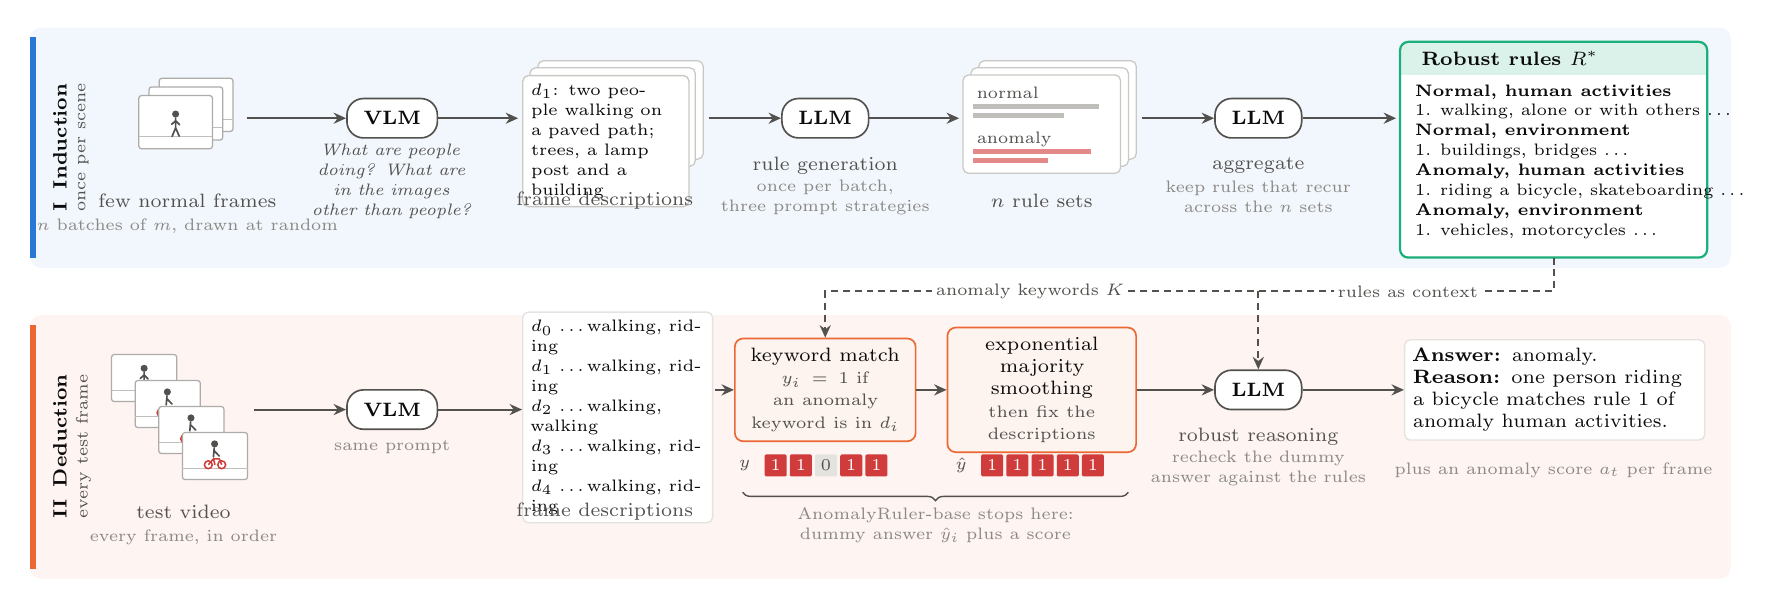
\begin{tikzpicture}[x=1cm,y=1cm]
\fill[indu!6,rounded corners=4pt] (0,0) rectangle (21.6,-3.05);
\fill[dedu!7,rounded corners=4pt] (0,-3.65) rectangle (21.6,-7.0);
\fill[indu] (0,-0.12) rectangle (0.08,-2.93);
\fill[dedu] (0,-3.77) rectangle (0.08,-6.88);
\node[rotate=90,font=\scriptsize\bfseries,text=ink] at (0.38,-1.52) {I\enspace Induction};
\node[rotate=90,font=\sixpt,text=ink2] at (0.68,-1.52) {once per scene};
\node[rotate=90,font=\scriptsize\bfseries,text=ink] at (0.38,-5.32) {II\enspace Deduction};
\node[rotate=90,font=\sixpt,text=ink2] at (0.68,-5.32) {every test frame};
% --- induction lane
\foreach \k in {2,1,0} \pic[scale=1.3] at ({1.85+\k*0.13},{-1.2+\k*0.11}) {vframe=walker};
\node[lbl] at (2.0,-2.2) {few normal frames};
\node[sublbl] at (2.0,-2.52) {$n$ batches of $m$, drawn at random};
\node[pill] (vlm1) at (4.6,-1.15) {VLM};
\draw[flow] (2.75,-1.15) -- (vlm1.west);
\node[font=\sixpt\itshape,text=ink2,text width=2.4cm,align=center] at (4.6,-1.95) {What are people doing? What are in the images other than people?};
\foreach \k in {2,1} \draw[grid!70!muted,fill=white,rounded corners=2pt,line width=0.45pt] ({6.25+\k*0.1},{-0.6+\k*0.09}) rectangle ++(2.1,-1.25);
\node[card=1.9cm,font=\sixpt,anchor=north west,minimum height=1.25cm,draw=grid!70!muted] (dsc) at (6.25,-0.6) {$d_1$: two people walking on a paved path; trees, a lamp post and a building};
\node[lbl] at (7.3,-2.2) {frame descriptions};
\draw[flow] (vlm1.east) -- (6.2,-1.15);
\node[pill] (gen) at (10.1,-1.15) {LLM};
\draw[flow] (8.62,-1.15) -- (gen.west);
\node[lbl] at (10.1,-1.75) {rule generation};
\node[sublbl] at (10.1,-2.15) {once per batch,\\three prompt strategies};
\foreach \k in {2,1} \draw[grid!70!muted,fill=white,rounded corners=2pt,line width=0.45pt] ({11.85+\k*0.1},{-0.6+\k*0.09}) rectangle ++(2.0,-1.25);
\draw[grid!70!muted,fill=white,rounded corners=2pt,line width=0.45pt] (11.85,-0.6) rectangle ++(2.0,-1.25);
\node[font=\sixpt,text=ink2,anchor=north west] at (11.9,-0.63) {normal};
\fill[muted!55] (11.98,-0.97) rectangle ++(1.6,-0.06); \fill[muted!55] (11.98,-1.09) rectangle ++(1.15,-0.06);
\node[font=\sixpt,text=ink2,anchor=north west] at (11.9,-1.2) {anomaly};
\fill[anom!60] (11.98,-1.54) rectangle ++(1.5,-0.06); \fill[anom!60] (11.98,-1.66) rectangle ++(0.95,-0.06);
\node[lbl] at (12.85,-2.2) {$n$ rule sets};
\draw[flow] (gen.east) -- (11.8,-1.15);
\node[pill] (agg) at (15.6,-1.15) {LLM};
\draw[flow] (14.12,-1.15) -- (agg.west);
\node[lbl] at (15.6,-1.75) {aggregate};
\node[sublbl] at (15.6,-2.15) {keep rules that recur\\across the $n$ sets};
\begin{scope}
  \clip[rounded corners=3pt] (17.4,-0.18) rectangle (21.3,-2.92);
  \fill[white] (17.4,-0.18) rectangle (21.3,-2.92);
  \fill[rulec!16] (17.4,-0.18) rectangle (21.3,-0.6);
\end{scope}
\draw[rulec,line width=0.8pt,rounded corners=3pt] (17.4,-0.18) rectangle (21.3,-2.92);
\node[font=\scriptsize\bfseries,text=ink,anchor=west] at (17.55,-0.39) {Robust rules $R^{*}$};
\node[font=\sixpt,text=ink,anchor=north west,align=left,inner sep=1pt] at (17.55,-0.68) {\textbf{Normal, human activities}\\1. walking, alone or with others \dots\\\textbf{Normal, environment}\\1. buildings, bridges \dots\\\textbf{Anomaly, human activities}\\1. riding a bicycle, skateboarding \dots\\\textbf{Anomaly, environment}\\1. vehicles, motorcycles \dots};
\draw[flow] (agg.east) -- (17.35,-1.15);
% --- deduction lane
\pic[scale=1.15] at (1.45,-4.45) {vframe=walker};
\pic[scale=1.15] at (1.75,-4.78) {vframe=cyclist};
\pic[scale=1.15] at (2.05,-5.11) {vframe=cyclist};
\pic[scale=1.15] at (2.35,-5.44) {vframe=cyclist};
\node[lbl] at (1.95,-6.15) {test video};
\node[sublbl] at (1.95,-6.47) {every frame, in order};
\node[pill] (vlm2) at (4.6,-4.85) {VLM};
\draw[flow] (2.85,-4.85) -- (vlm2.west);
\node[sublbl] at (4.6,-5.32) {same prompt};
\node[card=2.2cm,font=\sixpt,anchor=west] (dl) at (6.25,-4.95) {$d_0$ \dots walking, riding\\$d_1$ \dots walking, riding\\$d_2$ \dots walking, walking\\$d_3$ \dots walking, riding\\$d_4$ \dots walking, riding};
\draw[flow] (vlm2.east) -- (6.25,-4.85);
\node[lbl] at (7.3,-6.15) {frame descriptions};
\node[stage=dedu,text width=2.05cm] (km) at (10.1,-4.6) {keyword match\\{\sixpt\color{ink2}$y_i = 1$ if an anomaly keyword is in $d_i$}};
\draw[flow] (8.7,-4.6) -- (km.west);
\foreach \v [count=\k from 0] in {1,1,0,1,1} {
  \fill[c\v,rounded corners=0.5pt] ({9.33+\k*0.32},-5.42) rectangle ++(0.28,-0.28);
  \node[t\v,font=\sixpt] at ({9.47+\k*0.32},-5.56) {\v};}
\node[font=\sixpt,text=ink2,anchor=east] at (9.27,-5.56) {$y$};
\node[stage=dedu,text width=2.15cm] (ems) at (12.85,-4.6) {exponential majority smoothing\\{\sixpt\color{ink2}then fix the descriptions}};
\draw[flow] (km.east) -- (ems.west);
\foreach \v [count=\k from 0] in {1,1,1,1,1} {
  \fill[c\v,rounded corners=0.5pt] ({12.08+\k*0.32},-5.42) rectangle ++(0.28,-0.28);
  \node[t\v,font=\sixpt] at ({12.22+\k*0.32},-5.56) {\v};}
\node[font=\sixpt,text=ink2,anchor=east] at (12.02,-5.56) {$\hat y$};
\draw[decorate,decoration={brace,mirror,amplitude=3pt},draw=ink2,line width=0.5pt] (9.05,-5.9) -- (13.95,-5.9);
\node[sublbl] at (11.5,-6.32) {AnomalyRuler-base stops here:\\dummy answer $\hat y_i$ plus a score};
\node[pill] (rr) at (15.6,-4.6) {LLM};
\draw[flow] (ems.east) -- (rr.west);
\node[lbl] at (15.6,-5.2) {robust reasoning};
\node[sublbl] at (15.6,-5.6) {recheck the dummy\\answer against the rules};
\node[card=3.6cm,anchor=west] (out) at (17.45,-4.6) {\textbf{Answer:} anomaly.\\\textbf{Reason:} one person riding a bicycle matches rule 1 of anomaly human activities.};
\draw[flow] (rr.east) -- (out.west);
\node[sublbl,anchor=north] at (19.35,-5.4) {plus an anomaly score $a_t$ per frame};
% --- rules feed deduction
\draw[dflow] (19.35,-2.92) -- (19.35,-3.35) -- (10.1,-3.35) -- (km.north);
\draw[dflow] (15.6,-3.35) -- (rr.north);
\node[font=\sixpt,text=ink2,fill=white,inner sep=1.5pt] at (12.7,-3.35) {anomaly keywords $K$};
\node[font=\sixpt,text=ink2,fill=white,inner sep=1.5pt] at (17.5,-3.35) {rules as context};
\end{tikzpicture}
\par\vspace{7pt}
\textcol{6.95cm}{\textbf{Induction runs once per scene.} A VLM captions a few normal frames. An LLM
reads each caption, writes rules for normal, then flips them into rules for anomaly. This repeats
over $n$ random batches, and one last LLM call keeps only the rules that keep coming back.}\hfill
\textcol{6.95cm}{\textbf{Deduction runs on every frame.} The same VLM captions the test frame.
Matching the caption against anomaly keywords gives a first 0 or 1. Smoothing over neighbouring
frames cleans that guess, then an LLM rechecks it against the rules and writes the reason.}\hfill
\textcol{6.95cm}{\textbf{Paper setup.} CogVLM-17B captions frames, GPT-4 writes the rules, and the
open Mistral-7B runs deduction, since GPT-4 over whole test sets cost too much. Defaults are
$n = 10$, $m = 1$, $p = 5$, $\alpha = 0.33$. All models stay frozen.}
\end{minipage}
\\[8pt]
\midrule
% ---------------------------------------------------------------------
\cont{01 AnomalyRuler}{3 of 7}
&
\begin{minipage}[t]{\linewidth}
\rowhead{3}{Induction: from normal frames to a rule book}
\begin{minipage}[t]{10.75cm}
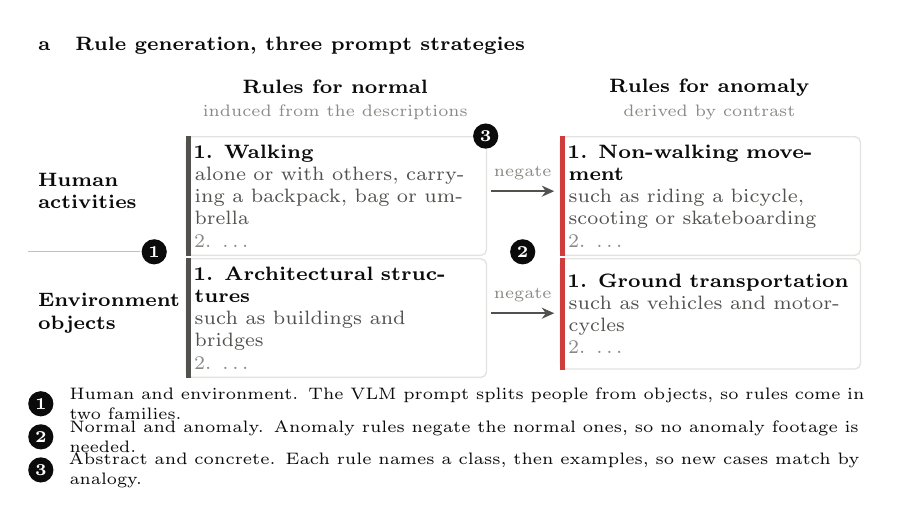
\begin{tikzpicture}[x=1cm,y=1cm]
\node[ptitle] at (0,0.25) {a\quad Rule generation, three prompt strategies};
\node[font=\scriptsize\bfseries,text=ink] at (3.9,-0.28) {Rules for normal};
\node[sublbl] at (3.9,-0.6) {induced from the descriptions};
\node[font=\scriptsize\bfseries,text=ink] at (8.65,-0.28) {Rules for anomaly};
\node[sublbl] at (8.65,-0.6) {derived by contrast};
\node[font=\scriptsize\bfseries,text=ink,anchor=west,align=left] at (0,-1.6) {Human\\activities};
\node[font=\scriptsize\bfseries,text=ink,anchor=west,align=left] at (0,-3.15) {Environment\\objects};
\node[card=3.6cm,minimum height=1.4cm,anchor=north west] (nh) at (2.0,-0.9) {\textbf{1. Walking}\\{\color{ink2}alone or with others, carrying a backpack, bag or umbrella}\\{\color{muted}2. \dots}};
\node[card=3.6cm,minimum height=1.4cm,anchor=north west] (ah) at (6.75,-0.9) {\textbf{1. Non-walking movement}\\{\color{ink2}such as riding a bicycle, scooting or skateboarding}\\{\color{muted}2. \dots}};
\node[card=3.6cm,minimum height=1.4cm,anchor=north west] (ne) at (2.0,-2.45) {\textbf{1. Architectural structures}\\{\color{ink2}such as buildings and bridges}\\{\color{muted}2. \dots}};
\node[card=3.6cm,minimum height=1.4cm,anchor=north west] (ae) at (6.75,-2.45) {\textbf{1. Ground transportation}\\{\color{ink2}such as vehicles and motorcycles}\\{\color{muted}2. \dots}};
\foreach \n in {nh,ne} \fill[ink2] (\n.north west) rectangle ([xshift=0.07cm]\n.south west);
\foreach \n in {ah,ae} \fill[anom] (\n.north west) rectangle ([xshift=0.07cm]\n.south west);
\draw[flow] (5.88,-1.6) -- (6.68,-1.6);
\draw[flow] (5.88,-3.15) -- (6.68,-3.15);
\node[sublbl,anchor=south] at (6.28,-1.58) {negate};
\node[sublbl,anchor=south] at (6.28,-3.13) {negate};
\node[badge] at (1.6,-2.37) {1};
\draw[grid!60!muted,line width=0.4pt] (0,-2.37) -- (1.42,-2.37);
\node[badge] at (6.28,-2.37) {2};
\node[badge] at (5.81,-0.9) {3};
\foreach \n/\txt [count=\r from 0] in {
  1/{Human and environment. The VLM prompt splits people from objects, so rules come in two families.},
  2/{Normal and anomaly. Anomaly rules negate the normal ones, so no anomaly footage is needed.},
  3/{Abstract and concrete. Each rule names a class, then examples, so new cases match by analogy.}}{
  \node[badge] at (0.16,{-4.3-\r*0.42}) {\n};
  \node[font=\sixpt,text=ink,anchor=west,text width=10.1cm] at (0.4,{-4.3-\r*0.42}) {\txt};
}
\end{tikzpicture}
\end{minipage}\hfill
\begin{minipage}[t]{10.6cm}
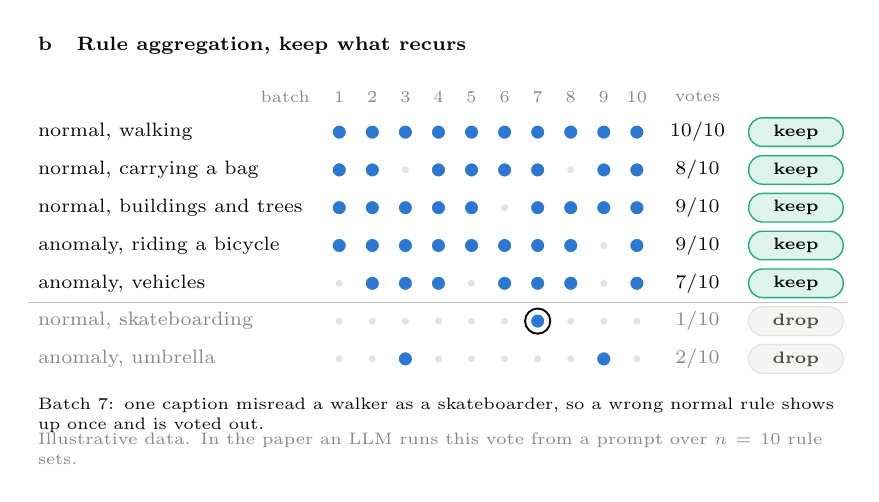
\begin{tikzpicture}[x=1cm,y=1cm]
\node[ptitle] at (0,0.25) {b\quad Rule aggregation, keep what recurs};
\node[font=\sixpt,text=muted,anchor=east] at (3.7,-0.4) {batch};
\foreach \j in {1,...,10} \node[font=\sixpt,text=muted] at ({3.95+(\j-1)*0.42},-0.4) {\j};
\node[font=\sixpt,text=muted] at (8.5,-0.4) {votes};
\foreach \lab/\pat/\cnt/\keep [count=\r from 0] in {
  {normal, walking}/{1,1,1,1,1,1,1,1,1,1}/10/1,
  {normal, carrying a bag}/{1,1,0,1,1,1,1,0,1,1}/8/1,
  {normal, buildings and trees}/{1,1,1,1,1,0,1,1,1,1}/9/1,
  {anomaly, riding a bicycle}/{1,1,1,1,1,1,1,1,0,1}/9/1,
  {anomaly, vehicles}/{0,1,1,1,0,1,1,1,0,1}/7/1,
  {normal, skateboarding}/{0,0,0,0,0,0,1,0,0,0}/1/0,
  {anomaly, umbrella}/{0,0,1,0,0,0,0,0,1,0}/2/0}{
  \pgfmathsetmacro\yy{-0.85-\r*0.48}
  \node[font=\scriptsize,k\keep,anchor=west] at (0,\yy) {\lab};
  \foreach \v [count=\j from 0] in \pat {
    \ifnum\v=1 \path[d1] ({3.95+\j*0.42},\yy) circle (0.095);
    \else \fill[grid] ({3.95+\j*0.42},\yy) circle (0.045); \fi}
  \node[font=\scriptsize,k\keep] at (8.5,\yy) {\cnt/10};
  \ifnum\keep=1 \node[tg-add] at (9.75,\yy) {keep};
  \else \node[tg-keep] at (9.75,\yy) {drop}; \fi
}
\draw[grid!60!muted,line width=0.4pt] (0,-3.01) -- (10.4,-3.01);
\draw[ink,line width=0.7pt] ({3.95+6*0.42},-3.25) circle (0.16);
\node[font=\sixpt,text=ink,anchor=north west,text width=10.2cm] at (0,-4.1) {Batch 7: one caption misread a walker as a skateboarder, so a wrong normal rule shows up once and is voted out.};
\node[font=\sixpt,text=muted,anchor=north west,text width=10.2cm] at (0,-4.55) {Illustrative data. In the paper an LLM runs this vote from a prompt over $n = 10$ rule sets.};
\end{tikzpicture}
\end{minipage}
\par\vspace{7pt}
\textcol{10.6cm}{Taking out the normal-to-anomaly contrast costs 18.8 AUC points on ShanghaiTech, the
biggest drop in the ablation. With normal rules alone the LLM flags walking with an umbrella as a
deviation and still misses real anomalies. Dropping the human and environment split halves the
rule count, from 42 to about 22, and costs 2.4 points.}\hfill
\textcol{10.6cm}{This is randomized smoothing applied to prompts. One bad caption can plant a wrong
rule, but the same mistake rarely repeats across ten independent batches. Without aggregation AUC
falls 15.8 points. More reference frames help up to a point: at $n = 20$, AUC slides from 85.9 to
72.2 as $m$ grows, because past about 100 frames the context gets too long.}
\end{minipage}
\\[8pt]
\midrule
% ---------------------------------------------------------------------
\cont{01 AnomalyRuler}{4 of 7}
&
\begin{minipage}[t]{\linewidth}
\rowhead{4}{Deduction, step one: perception smoothing on a toy video}
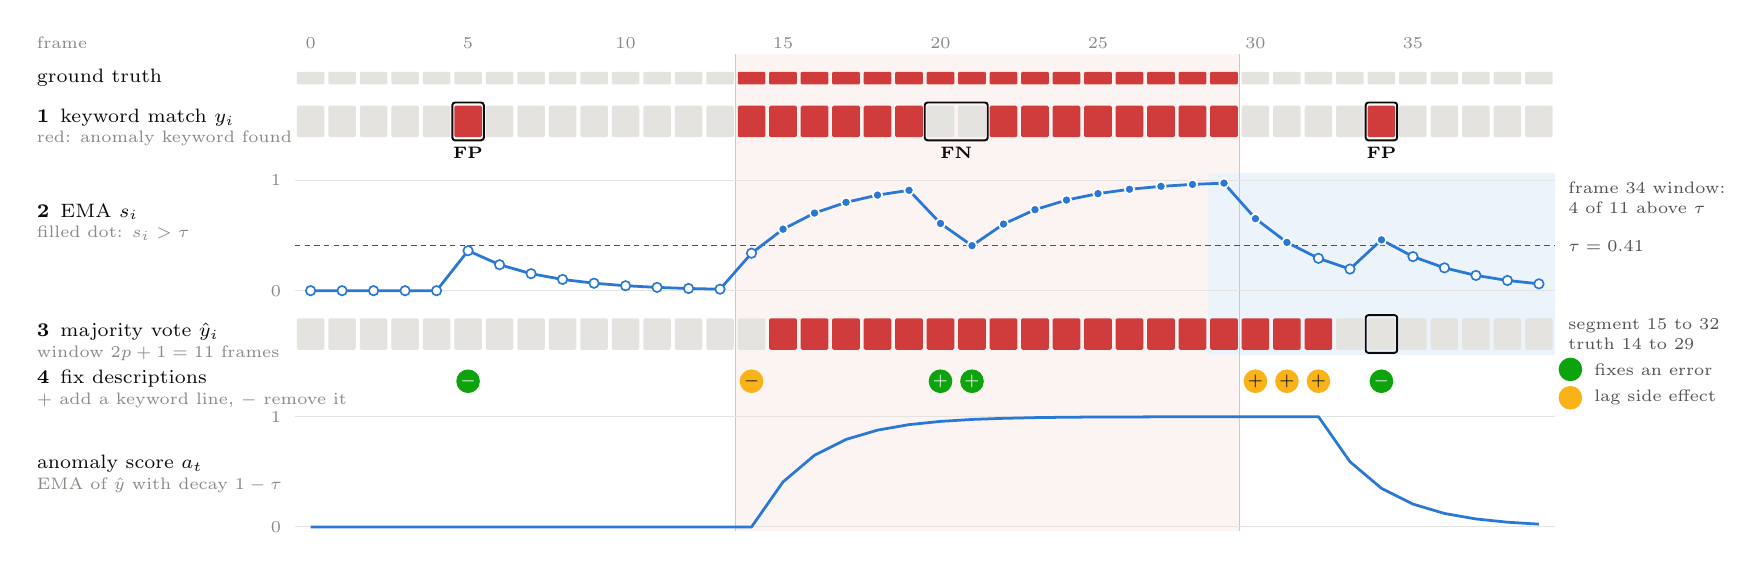
\begin{tikzpicture}[x=1cm,y=1cm]
\begin{scope}[on background layer]
  \fill[anom!6] (9.0,0.0) rectangle (15.4,-6.05);
  \fill[indu!9] (15.0,-1.5) rectangle (19.4,-3.82);
  \draw[anom!35,line width=0.4pt] (9.0,0.0) -- (9.0,-6.05) (15.4,0.0) -- (15.4,-6.05);
\end{scope}
\node[font=\sixpt,text=muted,anchor=west] at (0,0.15) {frame};
\foreach \k in {0,5,...,35} \node[font=\sixpt,text=muted] at ({3.6+\k*0.4},0.15) {\k};
% ground truth
\node[rowlab] at (0,-0.3) {ground truth};
\foreach \k in {0,...,39}{
  \pgfmathtruncatemacro\g{and(\k>13,\k<30)}
  \fill[c\g,rounded corners=0.4pt] ({3.425+\k*0.4},-0.22) rectangle ++(0.35,-0.16);}
% 1 keyword match
\node[rowlab] at (0,-0.8) {\textbf{1}\enspace keyword match $y_i$};
\node[rowsub] at (0,-1.07) {red: anomaly keyword found};
\foreach \v [count=\k from 0] in {0,0,0,0,0,1,0,0,0,0,0,0,0,0,1,1,1,1,1,1,0,0,1,1,1,1,1,1,1,1,0,0,0,0,1,0,0,0,0,0}
  \fill[c\v,rounded corners=0.5pt] ({3.425+\k*0.4},-0.65) rectangle ++(0.35,-0.4);
\foreach \k/\n in {5/1,20/2,34/1}
  \draw[ink,line width=0.7pt,rounded corners=1pt] ({3.4+\k*0.4},-0.61) rectangle ++({\n*0.4},-0.48);
\node[font=\sixpt\bfseries,text=ink] at (5.6,-1.25) {FP};
\node[font=\sixpt\bfseries,text=ink] at (11.8,-1.25) {FN};
\node[font=\sixpt\bfseries,text=ink] at (17.2,-1.25) {FP};
% 2 EMA
\node[rowlab] at (0,-2.0) {\textbf{2}\enspace EMA $s_i$};
\node[rowsub] at (0,-2.27) {filled dot: $s_i > \tau$};
\draw[grid,line width=0.4pt] (3.4,-3.0) -- (19.4,-3.0) (3.4,-1.6) -- (19.4,-1.6);
\node[font=\sixpt,text=muted,anchor=east] at (3.35,-3.0) {0};
\node[font=\sixpt,text=muted,anchor=east] at (3.35,-1.6) {1};
\draw[ink2,line width=0.5pt,dash pattern=on 2pt off 1.5pt] (3.4,-2.428) -- (19.4,-2.428);
\node[font=\sixpt,text=ink2,anchor=west] at (19.45,-2.428) {$\tau = 0.41$};
\node[font=\sixpt,text=ink2,anchor=north west,align=left] at (19.45,-1.5) {frame 34 window:\\4 of 11 above $\tau$};
\draw[indu,line width=1pt,line join=round] plot coordinates {(3.60,-3.000) (4.00,-3.000) (4.40,-3.000) (4.80,-3.000) (5.20,-3.000) (5.60,-2.492) (6.00,-2.670) (6.40,-2.784) (6.80,-2.857) (7.20,-2.905) (7.60,-2.937) (8.00,-2.958) (8.40,-2.972) (8.80,-2.981) (9.20,-2.524) (9.60,-2.219) (10.00,-2.014) (10.40,-1.878) (10.80,-1.786) (11.20,-1.725) (11.60,-2.146) (12.00,-2.428) (12.40,-2.154) (12.80,-1.971) (13.20,-1.849) (13.60,-1.767) (14.00,-1.712) (14.40,-1.675) (14.80,-1.650) (15.20,-1.634) (15.60,-2.085) (16.00,-2.387) (16.40,-2.589) (16.80,-2.725) (17.20,-2.354) (17.60,-2.567) (18.00,-2.710) (18.40,-2.806) (18.80,-2.870) (19.20,-2.913)};
\foreach \xx/\yy/\f in {3.60/-3.000/0,4.00/-3.000/0,4.40/-3.000/0,4.80/-3.000/0,5.20/-3.000/0,5.60/-2.492/0,6.00/-2.670/0,6.40/-2.784/0,6.80/-2.857/0,7.20/-2.905/0,7.60/-2.937/0,8.00/-2.958/0,8.40/-2.972/0,8.80/-2.981/0,9.20/-2.524/0,9.60/-2.219/1,10.00/-2.014/1,10.40/-1.878/1,10.80/-1.786/1,11.20/-1.725/1,11.60/-2.146/1,12.00/-2.428/1,12.40/-2.154/1,12.80/-1.971/1,13.20/-1.849/1,13.60/-1.767/1,14.00/-1.712/1,14.40/-1.675/1,14.80/-1.650/1,15.20/-1.634/1,15.60/-2.085/1,16.00/-2.387/1,16.40/-2.589/0,16.80/-2.725/0,17.20/-2.354/1,17.60/-2.567/0,18.00/-2.710/0,18.40/-2.806/0,18.80/-2.870/0,19.20/-2.913/0}
  \path[d\f] (\xx,\yy) circle (0.06);
% 3 majority vote
\node[rowlab] at (0,-3.52) {\textbf{3}\enspace majority vote $\hat y_i$};
\node[rowsub] at (0,-3.79) {window $2p+1 = 11$ frames};
\foreach \v [count=\k from 0] in {0,0,0,0,0,0,0,0,0,0,0,0,0,0,0,1,1,1,1,1,1,1,1,1,1,1,1,1,1,1,1,1,1,0,0,0,0,0,0,0}
  \fill[c\v,rounded corners=0.5pt] ({3.425+\k*0.4},-3.35) rectangle ++(0.35,-0.4);
\draw[ink,line width=0.7pt,rounded corners=1pt] (17.0,-3.31) rectangle ++(0.4,-0.48);
\node[font=\sixpt,text=ink2,anchor=west,align=left] at (19.45,-3.55) {segment 15 to 32\\truth 14 to 29};
% 4 description fix
\node[rowlab] at (0,-4.12) {\textbf{4}\enspace fix descriptions};
\node[rowsub] at (0,-4.39) {$+$ add a keyword line, $-$ remove it};
\foreach \k/\s/\ok in {5/-/1,14/-/0,20/+/1,21/+/1,30/+/0,31/+/0,32/+/0,34/-/1}
  \node[fx\ok] at ({3.6+\k*0.4},-4.15) {$\s$};
\node[fx1] at (19.6,-4.0) {};
\node[font=\sixpt,text=ink2,anchor=west] at (19.78,-4.0) {fixes an error};
\node[fx0] at (19.6,-4.36) {};
\node[font=\sixpt,text=ink2,anchor=west] at (19.78,-4.36) {lag side effect};
% score
\node[rowlab] at (0,-5.2) {anomaly score $a_t$};
\node[rowsub] at (0,-5.47) {EMA of $\hat y$ with decay $1-\tau$};
\draw[grid,line width=0.4pt] (3.4,-6.0) -- (19.4,-6.0) (3.4,-4.6) -- (19.4,-4.6);
\node[font=\sixpt,text=muted,anchor=east] at (3.35,-6.0) {0};
\node[font=\sixpt,text=muted,anchor=east] at (3.35,-4.6) {1};
\draw[indu,line width=1pt,line join=round] plot coordinates {(3.60,-6.000) (4.00,-6.000) (4.40,-6.000) (4.80,-6.000) (5.20,-6.000) (5.60,-6.000) (6.00,-6.000) (6.40,-6.000) (6.80,-6.000) (7.20,-6.000) (7.60,-6.000) (8.00,-6.000) (8.40,-6.000) (8.80,-6.000) (9.20,-6.000) (9.60,-5.428) (10.00,-5.090) (10.40,-4.889) (10.80,-4.771) (11.20,-4.701) (11.60,-4.660) (12.00,-4.635) (12.40,-4.621) (12.80,-4.612) (13.20,-4.607) (13.60,-4.604) (14.00,-4.603) (14.40,-4.602) (14.80,-4.601) (15.20,-4.601) (15.60,-4.600) (16.00,-4.600) (16.40,-4.600) (16.80,-5.172) (17.20,-5.510) (17.60,-5.710) (18.00,-5.829) (18.40,-5.899) (18.80,-5.940) (19.20,-5.965)};
\end{tikzpicture}
\par\vspace{6pt}
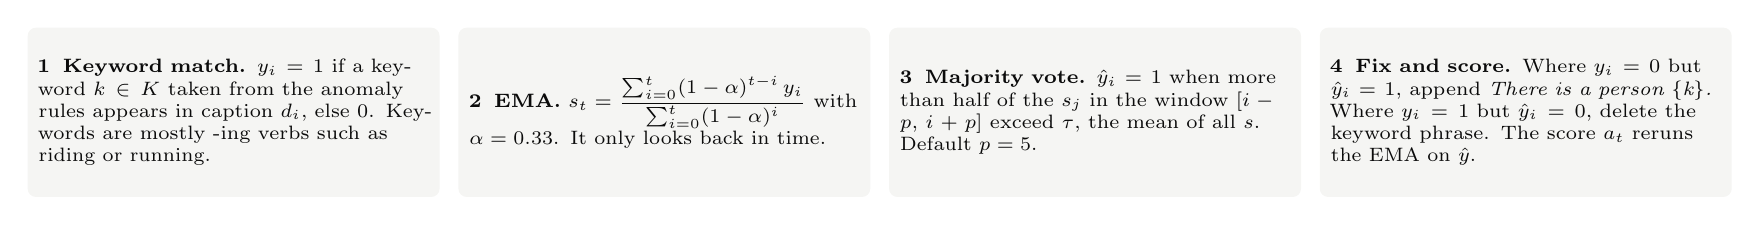
\begin{tikzpicture}[x=1cm,y=1cm]
\foreach \x/\txt in {
  0/{\textbf{1\enspace Keyword match.} $y_i = 1$ if a keyword $k \in K$ taken from the anomaly rules appears in caption $d_i$, else $0$. Keywords are mostly -ing verbs such as riding or running.},
  5.47/{\textbf{2\enspace EMA.} $\displaystyle s_t = \frac{\sum_{i=0}^{t} (1-\alpha)^{t-i}\, y_i}{\sum_{i=0}^{t} (1-\alpha)^{i}}$ with $\alpha = 0.33$. It only looks back in time.},
  10.94/{\textbf{3\enspace Majority vote.} $\hat y_i = 1$ when more than half of the $s_j$ in the window $[i-p,\, i+p]$ exceed $\tau$, the mean of all $s$. Default $p = 5$.},
  16.41/{\textbf{4\enspace Fix and score.} Where $y_i = 0$ but $\hat y_i = 1$, append \emph{There is a person \{k\}.} Where $y_i = 1$ but $\hat y_i = 0$, delete the keyword phrase. The score $a_t$ reruns the EMA on $\hat y$.}}
  \node[fill=panel,rounded corners=3pt,text width=4.95cm,minimum height=2.15cm,align=left,anchor=north west,inner sep=4pt,font=\scriptsize,text=ink] at (\x,0) {\txt};
\end{tikzpicture}
\par\vspace{7pt}
\textcol{10.6cm}{\textbf{What the toy run shows.} Forty frames, a true anomaly at frames 14 to 29, and
the paper's defaults $\alpha = 0.33$ and $p = 5$. Every curve and cell above comes from the paper's
formulas; only the input $y$ is made up. Smoothing removes both lone false positives and fills the
gap at frames 20 and 21. Frame 34 is the vote's job: its own EMA value clears $\tau$, but only 4 of
the 11 values in its window do.}\hfill
\textcol{10.6cm}{\textbf{The cost is lag.} The EMA only looks back, so the smoothed segment starts one
frame late and ends three late. Frames 30 to 32 get a fake keyword line and frame 14 loses a true
one. At 30 fps that is 0.1~s and does not matter. If we caption at 1 fps to fit the 5-minute
budget it grows to 3~s, and the brief scores timecode accuracy.}
\end{minipage}
\\[8pt]
\midrule
% ---------------------------------------------------------------------
\cont{01 AnomalyRuler}{5 of 7}
&
\begin{minipage}[t]{\linewidth}
\rowhead{5}{Deduction, step two: robust reasoning}
\begin{minipage}[t]{12.4cm}
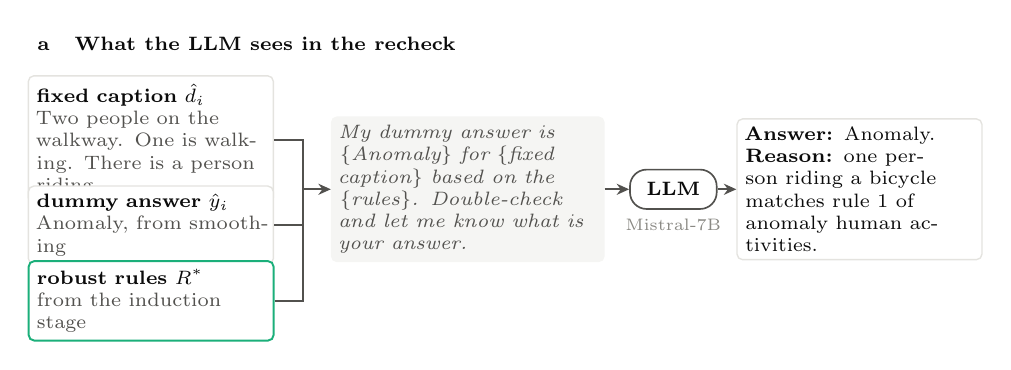
\begin{tikzpicture}[x=1cm,y=1cm]
\node[ptitle] at (0,0.25) {a\quad What the LLM sees in the recheck};
\node[card=2.9cm,anchor=north west] (in1) at (0,-0.15) {\textbf{fixed caption} $\hat d_i$\\{\color{ink2}Two people on the walkway. One is walking. There is a person riding.}};
\node[card=2.9cm,anchor=north west] (in2) at (0,-1.55) {\textbf{dummy answer} $\hat y_i$\\{\color{ink2}Anomaly, from smoothing}};
\node[card=2.9cm,anchor=north west,draw=rulec,line width=0.7pt] (in3) at (0,-2.5) {\textbf{robust rules} $R^{*}$\\{\color{ink2}from the induction stage}};
\node[card=3.25cm,anchor=west,fill=panel,draw=panel,font=\scriptsize\itshape,text=ink2] (pr) at (3.85,-1.6) {My dummy answer is \{Anomaly\} for \{fixed caption\} based on the \{rules\}. Double-check and let me know what is your answer.};
\draw[line width=0.7pt,draw=ink2] (in1.east) -| (3.5,-1.6) (in3.east) -| (3.5,-1.6) (in2.east) -- (in2.east -| 3.5,0);
\draw[flow] (3.5,-1.6) -- (pr.west);
\node[pill] (llm) at (8.2,-1.6) {LLM};
\node[sublbl] at (8.2,-2.05) {Mistral-7B};
\draw[flow] (pr.east) -- (llm.west);
\node[card=2.9cm,anchor=west] (out2) at (9.0,-1.6) {\textbf{Answer:} Anomaly.\\\textbf{Reason:} one person riding a bicycle matches rule 1 of anomaly human activities.};
\draw[flow] (llm.east) -- (out2.west);
\end{tikzpicture}
\end{minipage}\hfill
\begin{minipage}[t]{8.9cm}
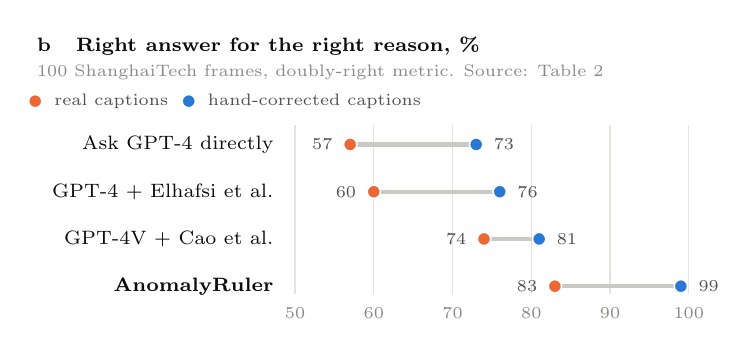
\begin{tikzpicture}[x=1cm,y=1cm]
\node[ptitle] at (0,0.25) {b\quad Right answer for the right reason, \%};
\node[font=\sixpt,text=muted,anchor=west] at (0,-0.08) {100 ShanghaiTech frames, doubly-right metric. Source: Table 2};
\path[d1,draw=white,fill=dedu] (0.1,-0.45) circle (0.085);
\node[font=\sixpt,text=ink2,anchor=west] at (0.22,-0.45) {real captions};
\path[d1] (2.05,-0.45) circle (0.085);
\node[font=\sixpt,text=ink2,anchor=west] at (2.17,-0.45) {hand-corrected captions};
\foreach \v in {50,60,...,100}{
  \draw[grid,line width=0.4pt] ({3.4+0.1*(\v-50)},-0.75) -- ({3.4+0.1*(\v-50)},-2.9);
  \node[font=\sixpt,text=muted,anchor=north] at ({3.4+0.1*(\v-50)},-2.95) {\v};}
\foreach \m/\a/\b/\bold [count=\r from 0] in {{Ask GPT-4 directly}/57/73/0,{GPT-4 + Elhafsi et al.}/60/76/0,{GPT-4V + Cao et al.}/74/81/0,{AnomalyRuler}/83/99/1}{
  \pgfmathsetmacro\yy{-1.0-\r*0.6}
  \ifnum\bold=1 \node[font=\scriptsize\bfseries,text=ink,anchor=east] at (3.25,\yy) {\m};
  \else \node[font=\scriptsize,text=ink,anchor=east] at (3.25,\yy) {\m}; \fi
  \draw[grid!70!muted,line width=1.6pt] ({3.4+0.1*(\a-50)},\yy) -- ({3.4+0.1*(\b-50)},\yy);
  \path[fill=dedu,draw=white,line width=0.6pt] ({3.4+0.1*(\a-50)},\yy) circle (0.085);
  \path[d1] ({3.4+0.1*(\b-50)},\yy) circle (0.085);
  \node[font=\sixpt,text=ink2,anchor=east] at ({3.4+0.1*(\a-50)-0.1},\yy) {\a};
  \node[font=\sixpt,text=ink2,anchor=west] at ({3.4+0.1*(\b-50)+0.1},\yy) {\b};
}
\end{tikzpicture}
\end{minipage}
\par\vspace{7pt}
\textcol{12.2cm}{The second LLM pass does not judge the frame from scratch. It gets the fixed caption,
the dummy answer from smoothing and the rules, and is told to double-check. The paper reports that
the hint cuts missed anomalies and ties each reason to a numbered rule. For AUC, Eq.~2 runs again on
these final answers to give the score.}\hfill
\textcol{8.9cm}{With hand-corrected captions AnomalyRuler is right for the right reason on 99 of 100
frames; with real captions, 83. Reasoning is not the weak link, perception is. Smoothing was off in
this test because the frames are not consecutive.}
\end{minipage}
\\[8pt]
\midrule
% ---------------------------------------------------------------------
\cont{01 AnomalyRuler}{6 of 7}
&
\begin{minipage}[t]{\linewidth}
\rowhead{6}{Results}
\begin{minipage}[t]{7.1cm}
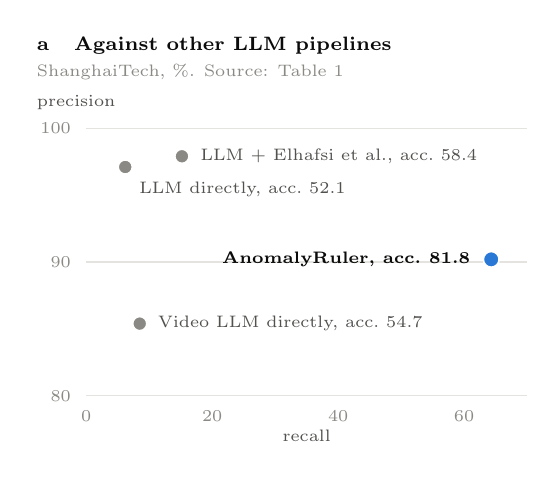
\begin{tikzpicture}[x=1cm,y=1cm]
\node[ptitle] at (0,4.45) {a\quad Against other LLM pipelines};
\node[font=\sixpt,text=muted,anchor=west] at (0,4.12) {ShanghaiTech, \%. Source: Table 1};
\node[font=\sixpt,text=ink2,anchor=west] at (0,3.72) {precision};
\foreach \p in {80,90,100}{
  \draw[grid,line width=0.4pt] (0.75,{0.17*(\p-80)}) -- (6.35,{0.17*(\p-80)});
  \node[font=\sixpt,text=muted,anchor=east] at (0.68,{0.17*(\p-80)}) {\p};}
\foreach \r in {0,20,40,60}
  \node[font=\sixpt,text=muted,anchor=north] at ({0.75+0.08*\r},-0.06) {\r};
\node[font=\sixpt,text=ink2] at (3.55,-0.5) {recall};
\foreach \r/\p in {6.2/97.1,15.2/97.9,8.5/85.4}
  \path[fill=muted,draw=white,line width=0.6pt] ({0.75+0.08*\r},{0.17*(\p-80)}) circle (0.09);
\path[d1] ({0.75+0.08*64.3},{0.17*(90.2-80)}) circle (0.1);
\node[font=\sixpt,text=ink2,anchor=west] at (2.08,3.043) {LLM + Elhafsi et al., acc.\ 58.4};
\node[font=\sixpt,text=ink2,anchor=north west] at (1.3,2.84) {LLM directly, acc.\ 52.1};
\node[font=\sixpt,text=ink2,anchor=west] at (1.54,0.918) {Video LLM directly, acc.\ 54.7};
\node[font=\sixpt\bfseries,text=ink,anchor=east] at (5.75,1.734) {AnomalyRuler, acc.\ 81.8};
\end{tikzpicture}
\end{minipage}\hfill
\begin{minipage}[t]{7.1cm}
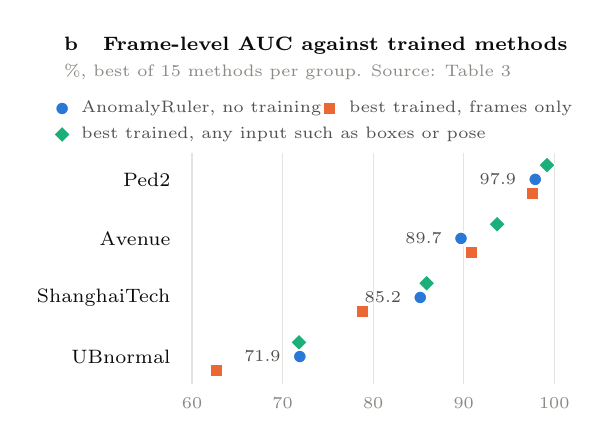
\begin{tikzpicture}[x=1cm,y=1cm]
\node[ptitle] at (0,4.45) {b\quad Frame-level AUC against trained methods};
\node[font=\sixpt,text=muted,anchor=west] at (0,4.12) {\%, best of 15 methods per group. Source: Table 3};
\path[d1] (0.1,3.65) circle (0.085);
\node[font=\sixpt,text=ink2,anchor=west] at (0.22,3.65) {AnomalyRuler, no training};
\path[fill=dedu,draw=white,line width=0.6pt] (3.5,3.65) +(-0.08,-0.08) rectangle +(0.08,0.08);
\node[font=\sixpt,text=ink2,anchor=west] at (3.62,3.65) {best trained, frames only};
\path[fill=rulec,draw=white,line width=0.6pt] (0.1,3.32) +(0,0.11) -- +(0.11,0) -- +(0,-0.11) -- +(-0.11,0) -- cycle;
\node[font=\sixpt,text=ink2,anchor=west] at (0.22,3.32) {best trained, any input such as boxes or pose};
\foreach \v in {60,70,80,90,100}{
  \draw[grid,line width=0.4pt] ({1.75+0.115*(\v-60)},0.15) -- ({1.75+0.115*(\v-60)},3.08);
  \node[font=\sixpt,text=muted,anchor=north] at ({1.75+0.115*(\v-60)},0.1) {\v};}
\foreach \d/\ar/\img/\any [count=\r from 0] in {Ped2/97.9/97.6/99.2,Avenue/89.7/90.9/93.7,ShanghaiTech/85.2/78.8/85.9,UBnormal/71.9/62.7/71.8}{
  \pgfmathsetmacro\yy{2.75-\r*0.75}
  \node[font=\scriptsize,text=ink,anchor=east] at (1.6,\yy) {\d};
  \path[fill=rulec,draw=white,line width=0.6pt] ({1.75+0.115*(\any-60)},\yy+0.18) +(0,0.11) -- +(0.11,0) -- +(0,-0.11) -- +(-0.11,0) -- cycle;
  \path[fill=dedu,draw=white,line width=0.6pt] ({1.75+0.115*(\img-60)},\yy-0.18) +(-0.08,-0.08) rectangle +(0.08,0.08);
  \path[d1] ({1.75+0.115*(\ar-60)},\yy) circle (0.085);
  \node[font=\sixpt,text=ink2,anchor=east] at ({1.75+0.115*(\ar-60)-0.12},\yy) {\ar};
}
\end{tikzpicture}
\end{minipage}\hfill
\begin{minipage}[t]{7.1cm}
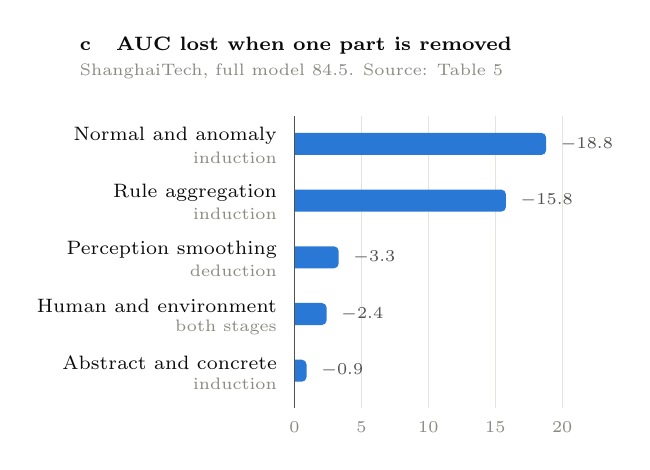
\begin{tikzpicture}[x=1cm,y=1cm]
\node[ptitle] at (0,4.45) {c\quad AUC lost when one part is removed};
\node[font=\sixpt,text=muted,anchor=west] at (0,4.12) {ShanghaiTech, full model 84.5. Source: Table 5};
\foreach \v in {0,5,10,15,20}{
  \draw[grid,line width=0.4pt] ({2.85+0.17*\v},-0.15) -- ({2.85+0.17*\v},3.55);
  \node[font=\sixpt,text=muted,anchor=north] at ({2.85+0.17*\v},-0.2) {\v};}
\foreach \n/\st/\v [count=\r from 0] in {{Normal and anomaly}/induction/18.8,{Rule aggregation}/induction/15.8,{Perception smoothing}/deduction/3.3,{Human and environment}/both stages/2.4,{Abstract and concrete}/induction/0.9}{
  \pgfmathsetmacro\yy{3.2-\r*0.72}
  \node[font=\scriptsize,text=ink,anchor=east] at (2.75,\yy+0.1) {\n};
  \node[font=\sixpt,text=muted,anchor=east] at (2.75,\yy-0.17) {\st};
  \hbarr{2.85}{\yy}{0.17*\v}
  \node[font=\sixpt,text=ink2,anchor=west] at ({2.85+0.17*\v+0.06},\yy) {$-$\v};
}
\draw[ink2,line width=0.5pt] (2.85,-0.15) -- (2.85,3.55);
\end{tikzpicture}
\end{minipage}
\par\vspace{7pt}
\textcol{7.0cm}{Asked directly, LLMs almost never say anomaly, so precision looks great and recall
sits at 6 to 15\%. AnomalyRuler finds 64\% of anomalous frames at 90\% precision.}\hfill
\textcol{7.0cm}{With no training it beats every frames-only method on Ped2, ShanghaiTech and
UBnormal, and trails the best one on Avenue by 1.2 points. Methods that add object boxes or pose
still lead on Ped2, Avenue and ShanghaiTech.}\hfill
\textcol{7.0cm}{Two parts carry the method: anomaly rules built by contrast, and the aggregation
vote. The other three add 0.9 to 3.3 points each. Rules induced on ShanghaiTech and applied to Ped2
reach 97.4 AUC with the base version, against 95.7 for zxVAD, Table~4.}
\end{minipage}
\\[8pt]
\midrule
% ---------------------------------------------------------------------
\cont{01 AnomalyRuler}{7 of 7}
&
\begin{minipage}[t]{\linewidth}
\rowhead{7}{What carries over to our ForteBank service}
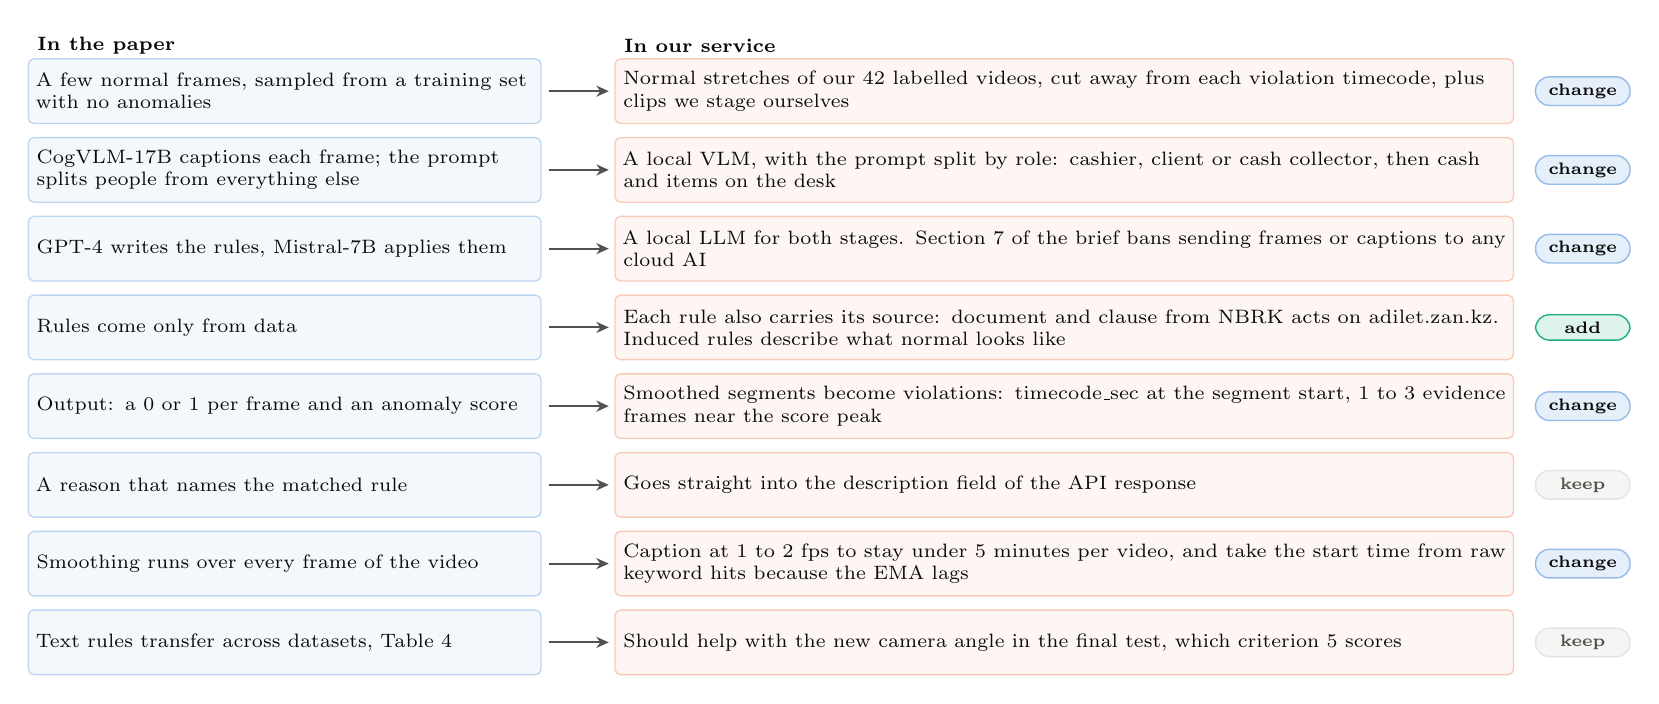
\begin{tikzpicture}[x=1cm,y=1cm]
\node[font=\scriptsize\bfseries,text=ink,anchor=west] at (0,-0.12) {In the paper};
\node[font=\scriptsize\bfseries,text=ink,anchor=west] at (7.45,-0.12) {In our service};
\foreach \p/\o/\t [count=\r from 0] in {
  {A few normal frames, sampled from a training set with no anomalies}/{Normal stretches of our 42 labelled videos, cut away from each violation timecode, plus clips we stage ourselves}/change,
  {CogVLM-17B captions each frame; the prompt splits people from everything else}/{A local VLM, with the prompt split by role: cashier, client or cash collector, then cash and items on the desk}/change,
  {GPT-4 writes the rules, Mistral-7B applies them}/{A local LLM for both stages. Section 7 of the brief bans sending frames or captions to any cloud AI}/change,
  {Rules come only from data}/{Each rule also carries its source: document and clause from NBRK acts on adilet.zan.kz. Induced rules describe what normal looks like}/add,
  {Output: a 0 or 1 per frame and an anomaly score}/{Smoothed segments become violations: timecode\_sec at the segment start, 1 to 3 evidence frames near the score peak}/change,
  {A reason that names the matched rule}/{Goes straight into the description field of the API response}/keep,
  {Smoothing runs over every frame of the video}/{Caption at 1 to 2 fps to stay under 5 minutes per video, and take the start time from raw keyword hits because the EMA lags}/change,
  {Text rules transfer across datasets, Table 4}/{Should help with the new camera angle in the final test, which criterion 5 scores}/keep}{
  \pgfmathsetmacro\yy{-0.7-\r*1.0}
  \node[card=6.3cm,anchor=west,minimum height=0.82cm,fill=indu!5,draw=indu!30] at (0,\yy) {\p};
  \draw[flow] (6.62,\yy) -- (7.38,\yy);
  \node[card=11.2cm,anchor=west,minimum height=0.82cm,fill=dedu!6,draw=dedu!35] at (7.45,\yy) {\o};
  \node[tg-\t] at (19.75,\yy) {\t};
}
\end{tikzpicture}
\par\vspace{8pt}
\textcol{10.6cm}{\textbf{Desk-level detail.} The paper's anomalies are people on bikes and cars in
outdoor scenes. Ours are hands, cash and documents seen from one camera above the till. If the VLM
cannot caption those, nothing downstream recovers.\par\vspace{4pt}
\textbf{Omissions.} Keyword matching flags something that is there. A cashier who skips a required
step leaves no keyword to match, so those rules need a check over a time window, not one frame.}\hfill
\textcol{10.6cm}{\textbf{One frame at a time.} Apart from smoothing, each frame is judged alone.
Actions that only make sense over a few seconds may need short clip captions instead.\par\vspace{4pt}
\textbf{False alarms.} The bank accepts no misses and wants few false alarms. The recheck targets
misses; the window $p$ and threshold $\tau$ decide how many false alarms survive, so tune them on our
42 labelled videos.}
\par\vspace{8pt}
{\small\textbf{Verdict.} Worth a prototype. Test VLM captions on five training clips first, since
everything depends on them. Then write the rule table with sources, then add smoothing and the recheck.}
\end{minipage}
\\[8pt]

% =====================================================================
% Template for the next paper. Copy, uncomment, and fill in.
% =====================================================================
% \midrule
% \begin{minipage}[t]{\linewidth}\raggedright
% {\fontsize{22}{24}\selectfont\bfseries\color{grid!50!muted}02}\par\vspace{5pt}
% {\small\bfseries\href{papers/FILE.pdf}{TITLE}}\par\vspace{5pt}
% {\scriptsize\color{ink2}AUTHORS\par}
% \vspace{4pt}{\scriptsize\bfseries VENUE YEAR}\par\vspace{8pt}
% {\scriptsize\href{papers/FILE.pdf}{\faFilePdf\enspace local copy}\par
%  \href{URL}{\faGlobe\enspace online}\par}
% \end{minipage}
% &
% \begin{minipage}[t]{\linewidth}
% \rowhead{1}{HEADING}
% % tikzpicture here, at most 21.5 cm wide
% \end{minipage}
% \\[8pt]

\end{longtable}

\end{document}
